\documentclass{standalone}
\usepackage{tikz}
\usepackage{amsmath}

\begin{document}
\boxed{
	\begin{tikzpicture}[scale=.6]
		\draw (1,3.7) to (1,3);

		\draw (1,3) to [out=205, in=90] (0,0);

		\draw [shorten >= 0cm] (.6,2.73) to [out=-100, in=90] (2,0);

		\draw [shorten >= .15cm] (1,3) to [out=-25, in=30, distance=1.1cm] (1,1.5);
		\draw [shorten <= .1cm] (1,1.5) to [out=210, in=20] (0,1);

		\node at (1,3.9){};
		\node at (0,-.32){};
		\node at (2,-.32){};

		\node at (3,1.5){$\sim$\ \ \ };
	\end{tikzpicture}
	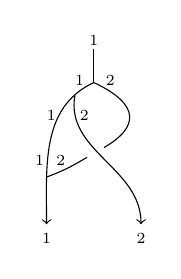
\begin{tikzpicture}[scale=.6]
		\draw (1,3.7) to (1,3);

		\draw [->](1,3) to [out=205, in=90] (0,0);

		\draw [shorten >= 0cm,->] (.6,2.73) to [out=-100, in=90] (2,0);

		\draw [shorten >= .15cm] (1,3) to [out=-25, in=30, distance=1.1cm] (1,1.5);
		\draw [shorten <= .1cm] (1,1.5) to [out=210, in=20] (0,1);

		\def\x{.8}

		\node[scale=\x] at (1,3.9){$\scriptstyle 1$};

		\node[scale=\x] at (.7,3.05){$\scriptstyle 1$};
		\node[scale=\x] at (1.35,3.05){$\scriptstyle 2$};

		\node[scale=\x] at (.1,2.3){$\scriptstyle 1$};
		\node[scale=\x] at (.8,2.3){$\scriptstyle 2$};

		\node[scale=\x] at (-.15,1.35){$\scriptstyle 1$};
		\node[scale=\x] at (.3,1.35){$\scriptstyle 2$};

		\node[scale=\x] at (0,-.3){$\scriptstyle 1$};
		\node[scale=\x] at (2,-.3){$\scriptstyle 2$};
	\end{tikzpicture}
}
\end{document}